\documentclass[11pt]{opticajnl}
\journal{opticajournal} % use for journal or Optica Open submissions

% See template introduction for guidance on setting shortarticle option
\setboolean{shortarticle}{true}
% true = letter/tutorial
% false = research/review article

% ONLY applicable for journal submission shortarticle types:
% When \setboolean{shortarticle}{true}
% then \setboolean{memo}{true} will print "Memorandum" on title page header
% Otherwise header will remain as "Letter"
% \setboolean{memo}{true}
\usepackage{lineno}
\usepackage{listings}
\usepackage{color}  % Para colorear el código
\usepackage[outputdir=build]{minted}


\definecolor{dkgreen}{rgb}{0,0.6,0}
\definecolor{gray}{rgb}{0.5,0.5,0.5}
\definecolor{mauve}{rgb}{0.58,0,0.82}
\lstset{language=SQL,
  basicstyle={\small\ttfamily},
  belowskip=3mm,
  breakatwhitespace=true,
  breaklines=true,
  classoffset=0,
  columns=flexible,
  commentstyle=\color{dkgreen},
  framexleftmargin=0.25em,
  frameshape={}{yy}{}{}, %To remove to vertical lines on left, set `frameshape={}{}{}{}`
  keywordstyle=\color{blue},
  numbers=none, %If you want line numbers, set `numbers=left`
  numberstyle=\tiny\color{gray},
  showstringspaces=false,
  stringstyle=\color{dkgreen},
  tabsize=3,
  xleftmargin =1em, 
  literate={'}{{\texttt{'}}}1
  		   {"}{{\texttt{"}}}1
}



\lstdefinestyle{terminal}{
  backgroundcolor=\color{white},   % Fondo blanco
  basicstyle=\color{black}\ttfamily, % Texto negro en fuente monoespaciada
  keywordstyle=\color{black}\bfseries, % Palabras clave en azul y negrita
  commentstyle=\color{black}\ttfamily, % Comentarios en verde
  stringstyle=\color{black}\ttfamily, % Cadenas en rojo
  morekeywords={sudo, apt-get, install, cd, ls, mkdir, rm, rmdir, cp, mv, echo, cat, nano, vim, grep, find, chmod, chown, systemctl, service, update, upgrade, reboot, shutdown, exit}, % Comandos comunes de terminal
  breaklines=true, % Permitir saltos de línea
  frame=single, % Marco alrededor del código
  framerule=0.5pt, % Grosor del marco
  rulecolor=\color{gray}, % Color del marco
  xleftmargin=0.05\textwidth, % Margen izquierdo
  xrightmargin=0.05\textwidth, % Margen derecho
  aboveskip=1em, % Espacio antes del bloque de código
  belowskip=1em % Espacio después del bloque de código
}

% Definir el lenguaje Cypher
\lstdefinelanguage{Cypher}{
  keywords={
    MATCH, RETURN, WHERE, CREATE, DELETE, SET, MERGE, 
    WITH, UNION, UNION ALL, LOAD CSV, USING, INDEX,
    START, FOREACH, ON, WHEN, CASE, THEN, ELSE, END,
    SKIP, LIMIT, ORDER BY, DESC, ASC, IN, AND, OR, NOT,
    CONTAINS, DISTINCT, OPTIONAL, DETACH, EXISTS,
    CONSTRAINT, ASSERT, UNIQUE, DROP, REMOVE, ORDER, BY
  },
  sensitive=true,
  comment=[l]//,
  morecomment=[s]{/*}{*/},
  morestring=[b]',
  morestring=[b]"
}


%\linenumbers % Turn off line numbering for Optica Open preprint submissions.

\title{Trabajo de prácticas BDGE}

\author[1,2,3]{Luis Ardévol Mesa, Miguel Mato Martínez}


\begin{abstract}
Usando una conjunto de datos de partidos de tenis, se usarán distintos tipos de base de datos para realizar consultas acerca de los mismos. En concreto, se tratarán bases de datos relaciones y con datos agregados en PostgreSQL, bases de datos distribuidas con SQL usando CITUS Data, y dos tipos de bases de datos noSQL: documentales con MongoDB y en grafo con Neo4j.
\end{abstract}

\setboolean{displaycopyright}{false} % Do not include copyright or licensing information in submission.

\begin{document}

\maketitle

\section{Bases de datos relacionales (PostgreSQL)}

\begin{figure}[H]
  \centering
  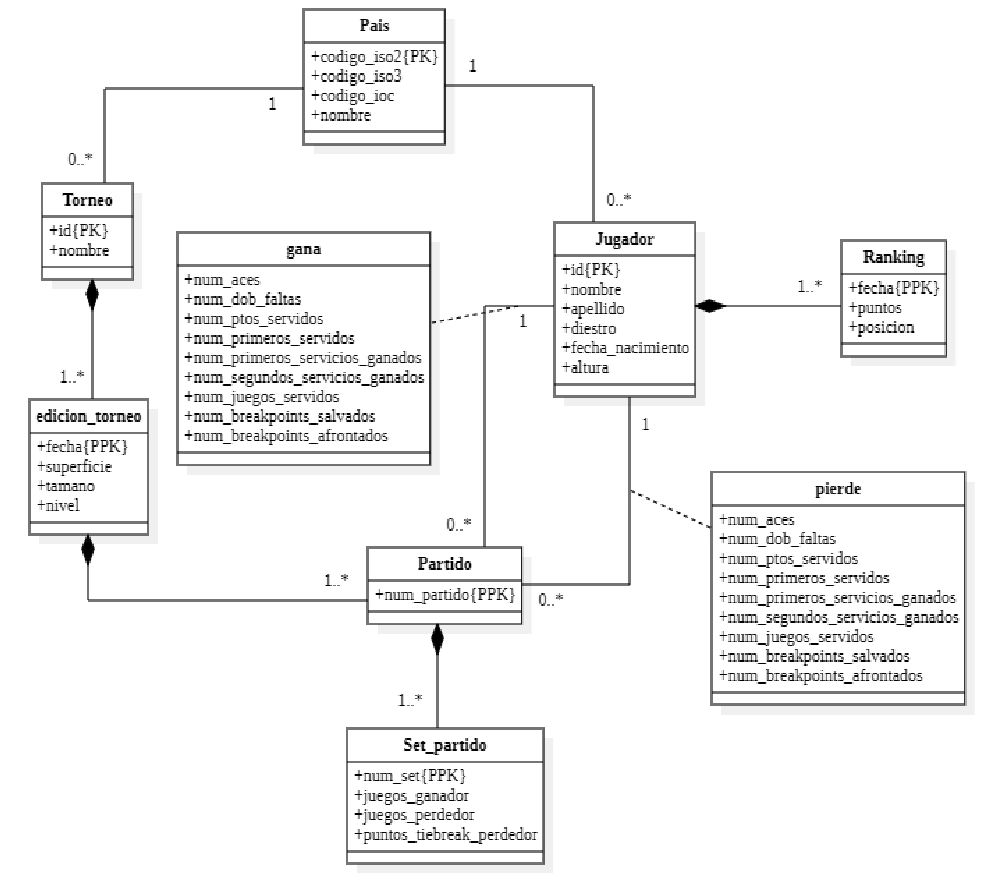
\includegraphics[width=0.7\textwidth]{fotos/esquema.png}
  \caption{Esquema de la base de datos de partidos de tenis.}
  \label{fig:schbd}
\end{figure}

En la figura \ref{fig:schbd} se muestra el esquema de la base de datos de partidos de tenis. Comenzaremos explicando este esquema de forma breve, pero haciendo especial hincapié en las relaciones entre las distintas tablas, ya que esto ayudará a comprender mejor las condiciones de \textit{join} a usar en las consultas que usen este esquema. Destacamos que no se hará uso de la tabla \texttt{ranking}, por lo que no se comentará en el siguiente análisis. \\

La tabla \texttt{pais} contiene la información relativa a países, y se usará tanto para mostrar el país dónde se celebra un torneo como para referenciar el país de procedencia de un jugador; su clave primaria es \texttt{codigo\_iso2}. La tabla \texttt{jugador} contiene la información de los jugadores, y su clave primaria es el \texttt{id} de cada jugador; el atributo \texttt{pais} referencia a \texttt{pais(codigo\_iso2)}. La tabla \texttt{torneo} contiene la información de los torneos; su clave primaria es el \texttt{id} de cada torneo y el atributo \texttt{pais} referencia a \texttt{pais(codigo\_iso2)}. La tabla \texttt{edicion\_torneo} contiene la información de las ediciones de los torneos; su clave primaria es una combinación de los atributos \texttt{torneo} y \texttt{fecha}, donde el atributo \texttt{torneo} es una referencia a \texttt{torneo(id)}. La tabla \texttt{partido} contiene la información de los partidos disputados; su clave primaria es la combinación de los atributos \texttt{torneo}, \texttt{fecha} y \texttt{num\_partido}, y tiene una clave foránea compuesta por los atributos \texttt{torneo} y \texttt{fecha}, que referencia a la clave primaria de \texttt{edicion\_torneo}, \texttt{edicion\_torneo(torneo, fecha)}. Además, los atributos \texttt{ganador} y \texttt{perdedor} son los \texttt{id} de los jugadores, por lo que puede enlazarse esta tabla con la de \texttt{jugador} mediante \texttt{jugador(id)}. Por último, la tabla \texttt{sets\_partido} contiene la información de los sets de los partidos; su clave primaria es la combinación de los atributos \texttt{torneo}, \texttt{fecha}, \texttt{num\_partido} y \texttt{num\_set}, y tiene una clave foránea compuesta por los atributos \texttt{torneo}, \texttt{fecha} y \texttt{num\_partido}, que referencia a la clave primaria de \texttt{partido}, \texttt{partido(torneo, fecha, num\_partido)}. \\

Tras ver cómo se estructura la base de datos a usar, creamos la base de datos en PostgreSQL y cargamos los datos en ella. La estructura relacional se proporciona en el archivo \texttt{schema.sql}, y los datos en los archivos \texttt{pais.csv}, \texttt{jugador.csv}, \texttt{torneo.csv}, \texttt{edicion\_torneo.csv}, \texttt{partido.csv}, \texttt{sets\_partido.csv} y \texttt{ranking.csv}. Una vez creada la base de datos \texttt{tenis}, ejecutamos el archivo \texttt{schema.sql} con la definición de los esquemas de las tablas mediante el siguiente comando en la terminal:

\begin{lstlisting}[style=terminal]
psql -U alumnogreibd -d tenis -f /home/alumnogreibd/BDGE/datos/datos_tenis/schema.sql
\end{lstlisting}

Ahora, con los esquemas definidos (pero vacíos), cargamos los datos a partir de los archivos \texttt{.csv} con los siguientes comandos en terminal (es importante seguir el orden de carga de los datos debido a las dependencias entre las tablas):

\begin{lstlisting}[style=terminal]
psql -U alumnogreibd -d tenis -c "\copy pais from /home/alumnogreibd/BDGE/datos/datos_tenis/pais.csv csv"
psql -U alumnogreibd -d tenis -c "\copy jugador from /home/alumnogreibd/BDGE/datos/datos_tenis/jugador.csv csv"
psql -U alumnogreibd -d tenis -c "\copy torneo from /home/alumnogreibd/BDGE/datos/datos_tenis/torneo.csv csv"
psql -U alumnogreibd -d tenis -c "\copy edicion_torneo from /home/alumnogreibd/BDGE/datos/datos_tenis/edicion_torneo.csv csv"
psql -U alumnogreibd -d tenis -c "\copy partido from /home/alumnogreibd/BDGE/datos/datos_tenis/partido.csv csv"
psql -U alumnogreibd -d tenis -c "\copy sets_partido from /home/alumnogreibd/BDGE/datos/datos_tenis/sets_partido.csv csv"
psql -U alumnogreibd -d tenis -c "\copy ranking from /home/alumnogreibd/BDGE/datos/datos_tenis/ranking.csv csv"
\end{lstlisting}

Este orden es lógico por las dependencias entre tablas que comentamos anteriormente: \texttt{sets\_partido} referencia a \texttt{partido}, por lo que es necesario cargar primero los datos de \texttt{partido} para poder cargar los de \texttt{sets\_partido}. Este razonamiento aplica al resto de tablas: \texttt{partido} referencia a \texttt{edicion\_torneo}, que referencia a \texttt{torneo}, que a su vez referencia a \texttt{pais}, que es referenciado por \texttt{jugador}. \\

En las siguientes consultas, los \textit{join} se harán mediante \textit{theta join} (\textit{inner} por defecto). En caso de que se quiera hacer otro tipo de \textit{join}, se especificará de forma clara en la consulta. Esto considera el producto cartesiano de las tablas a unir y selecciona solo las tuplas que verifiquen el predicado (la condición o condiciones de \textit{join}). Estos \textit{join} se harán de forma general de forma implícita en la claúsula \texttt{where}, siguiendo los atributos referenciados entre las tablas. Además, trabajaremos siempre dentro del mismo esquema. \\


\subsubsection{Muestra todos los ganadores del torneo ``Wimbledon'' (Nombre, apellidos y año). Ordena el resultado por año.}

Para esta consulta necesitamos la información de los jugadores, los partidos y los torneos, por lo que comenzamos en el \texttt{from} con el producto cartesiano de las tablas \texttt{jugador}, \texttt{partido} y \texttt{torneo} (especificando un alias para cada una de ellas). A continuación, especificamos las condiciones de \textit{join} en el \texttt{where}, así como otras condiciones de selección: 
\begin{itemize}
\item Condiciones de \textit{join}:
\begin{itemize}
\item El predicado \texttt{j.id = p.ganador} sirve para unir la tabla \texttt{jugador} con la tabla \texttt{partido} mediante el atributo \texttt{id} de la tabla \texttt{jugador} y el atributo \texttt{ganador} de la tabla \texttt{partido}, haciendo una selección únicamente de las tuplas que cumplan esta condición. Esto nos permite, para cada jugador, seleccionar solo los partidos en los que ha ganado.
\item El predicado \texttt{t.id = p.torneo} sirve para unir la tabla \texttt{torneo} con la tabla \texttt{partido} mediante el atributo \texttt{id} de la tabla \texttt{torneo} y el atributo \texttt{torneo} de la tabla \texttt{partido}, haciendo una selección únicamente de las tuplas que cumplan esta condición. Esto nos permite seleccionar solo los partidos que se han jugado en un torneo concreto.
\end{itemize}
\item Condiciones de selección:
\begin{itemize}
\item La condición \texttt{t.nombre = `Wimbledon'} selecciona solo el torneo cuyo nombre es ``Wimbledon''. Al hacer el \textit{join} con la tabla \texttt{torneo}, estamos seleccionando solo los partidos que se han jugado en el torneo ``Wimbledon''.
\item La condición \texttt{p.ronda = `F'} selecciona solo los partidos que han sido finales.
\end{itemize}
\end{itemize}

Tras seleccionar las tuplas que nos interesan, usamos el \texttt{select} para obtener la proyección de las filas que nos interesan: en esta caso, nos quedamos con los atributos \texttt{nombre} y \texttt{apellido} de la tabla \texttt{jugador} y el año de la fecha del partido, que denotaremos por el alias ``ano''. Como \texttt{p.fecha} es del tipo \texttt{date}, este último atributo lo obtenemos mediante la función \texttt{extract()}, especificando que solo queremos el año de ese atributo (\texttt{year from p.fecha}). Tras esto, ordenamos el resultado por año con \texttt{order by ano}; el orden por defecto es ascendente. El código de la consulta se muestra a continuación, y el resultado se pueden ver en la figura \ref{fig:q1_rel}.

\begin{minted}[frame=single, fontsize=\footnotesize]{sql}
select j.nombre, j.apellido, extract(year from p.fecha) as ano
from jugador j, partido p, torneo t
where j.id = p.ganador 
  and t.id = p.torneo 
  and t.nombre = 'Wimbledon' 
  and p.ronda = 'F'
order by ano
\end{minted}

\begin{figure}[H]
\centering
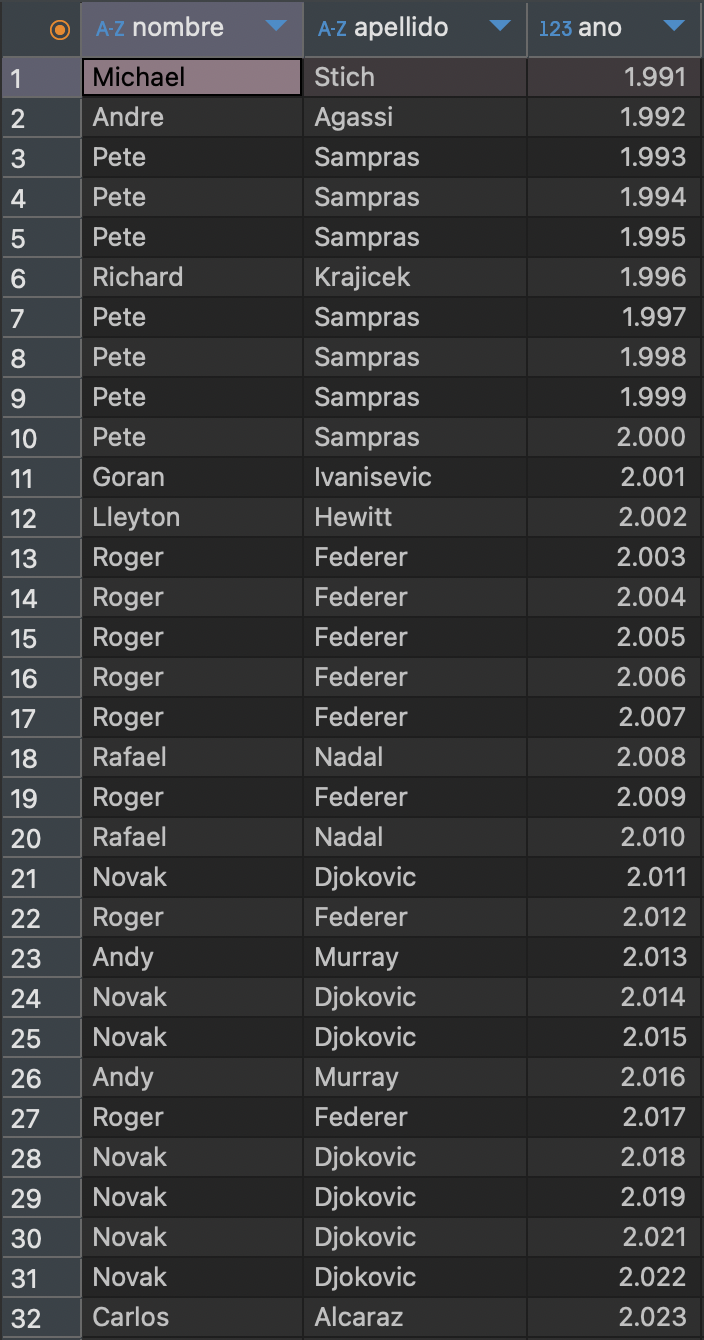
\includegraphics[height=0.4\textheight]{fotos/q1_rel.png}
\caption{Modelo relacional Postgresql, consulta 1.}
\label{fig:q1_rel}
\end{figure}



\subsubsection{Muestra los años en los que Roger Federer ganó algún torneo de nivel Gran Slam (G) o Master 1000 (M). Para cada año, muestra el número de torneos y lista sus nombres (ordenados por la fecha de celebración). Ordena el resultado por el año}

Para esta consulta necesitamos información de los jugadores, los partidos, los torneos y las ediciones de los torneos. Comenzamos en el \texttt{from} con el producto cartesiano de las tablas \texttt{jugador}, \texttt{partido}, \texttt{torneo} y \texttt{edicion\_torneo} (especificando un alias para cada una de ellas). A continuación, especificamos las condiciones de \textit{join} en el \texttt{where}, así como otras condiciones de selección:
\begin{itemize}
\item Condiciones de \textit{join} que, en global, nos permitirán seleccionar las tuplas de un jugador específico que ganó un torneo específico en un año específico:
\begin{itemize}
\item El predicado \texttt{j.id = p.ganador} sirve para unir la tabla \texttt{jugador} con la tabla \texttt{partido} mediante el atributo \texttt{id} de la tabla \texttt{jugador} y el atributo \texttt{ganador} de la tabla \texttt{partido}, haciendo una selección únicamente de las tuplas que cumplan esta condición. Esto nos permite, para cada jugador, seleccionar solo los partidos en los que ha ganado.
\item El predicado \texttt{t.id = p.torneo} sirve para unir la tabla \texttt{torneo} con la tabla \texttt{partido} mediante el atributo \texttt{id} de la tabla \texttt{torneo} y el atributo \texttt{torneo} de la tabla \texttt{partido}, haciendo una selección únicamente de las tuplas que cumplan esta condición. Esto nos permite seleccionar solo los partidos que se han jugado en un torneo concreto.
\item El predicado \texttt{t.id = et.torneo} sirve para unir la tabla \texttt{torneo} con la tabla \texttt{edicion\_torneo} mediante el atributo \texttt{id} de la tabla \texttt{torneo} y el atributo \texttt{torneo} de la tabla \texttt{edicion\_torneo}, haciendo una selección únicamente de las tuplas que cumplan esta condición. Esto nos permite seleccionar ediciones de torneos concretos.
\item El predicado \texttt{p.fecha = et.fecha} sirve para unir la tabla \texttt{partido} con la tabla \texttt{edicion\_torneo} mediante el atributo \texttt{fecha} de la tabla \texttt{partido} y el atributo \texttt{fecha} de la tabla \texttt{edicion\_torneo}, haciendo una selección únicamente de las tuplas que cumplan esta condición. Esto nos permite seleccionar solo los partidos que se han jugado en una edición concreta de un torneo (concreto, por la condición anterior).
\end{itemize}
\item Estamos interesados específicamente en torneos de nivel Gran Slam (G) o Master 1000 (M) y en las finales ganadas por Roger Federer (lo que indica que ganó el torneo) durante varios años (es decir, varias ediciones de torneos). Por tanto, las condiciones de selección son:
\begin{itemize}
\item El predicado \texttt{p.ronda = 'F'} selecciona solo los partidos que han sido finales.
\item El predicado \texttt{j.nombre = 'Roger' and j.apellido = 'Federer'} selecciona solo los partidos en los que ha ganado ``Roger Federer''.
\item El predicado \texttt{et.nivel in ('G', 'M')} selecciona solo los torneos de nivel Gran Slam (G) o Master 1000 (M).
\end{itemize}
\end{itemize}

Con el \texttt{group by} agrupamos los resultados por el año en que se celebraron los torneos, para su posterior concatenación. Por último, obtenemos la proyección de los atributos que nos interesan: el año, que lo obtenemos extrayendo el año de la fecha de celebración del partido; el número de torneos ganados, que lo obtenemos contando el número de torneos distintos (usamos el \texttt{id} del torneo para diferenciar) en el resultado agrupado por año (\texttt{count(distinct t.id)}). Como última proyección, obtenemos una concantenación (con \texttt{string\_agg()}) de esos torneos, separados por comas y ordenados por fecha de celebración de esa edición, en orden ascendente (\texttt{order by et.fecha}). El código de la consulta se muestra a continuación, y el resultado se pueden ver en la figura \ref{fig:q2_rel}.

\begin{minted}[frame=single, fontsize=\footnotesize]{sql}
select extract(year from et.fecha) as ano, count(distinct t.id) as numero_torneos, 
	string_agg(t.nombre, ', ' order by et.fecha) as torneos
from jugador j, partido p, torneo t, edicion_torneo et
where j.id = p.ganador
  and t.id = et.torneo
  and p.torneo = t.id
  and p.fecha = et.fecha
  and p.ronda = 'F'
  and j.nombre = 'Roger'
  and j.apellido = 'Federer'
  and et.nivel in ('G', 'M')
group by ano
\end{minted}

\begin{figure}[H]
\centering
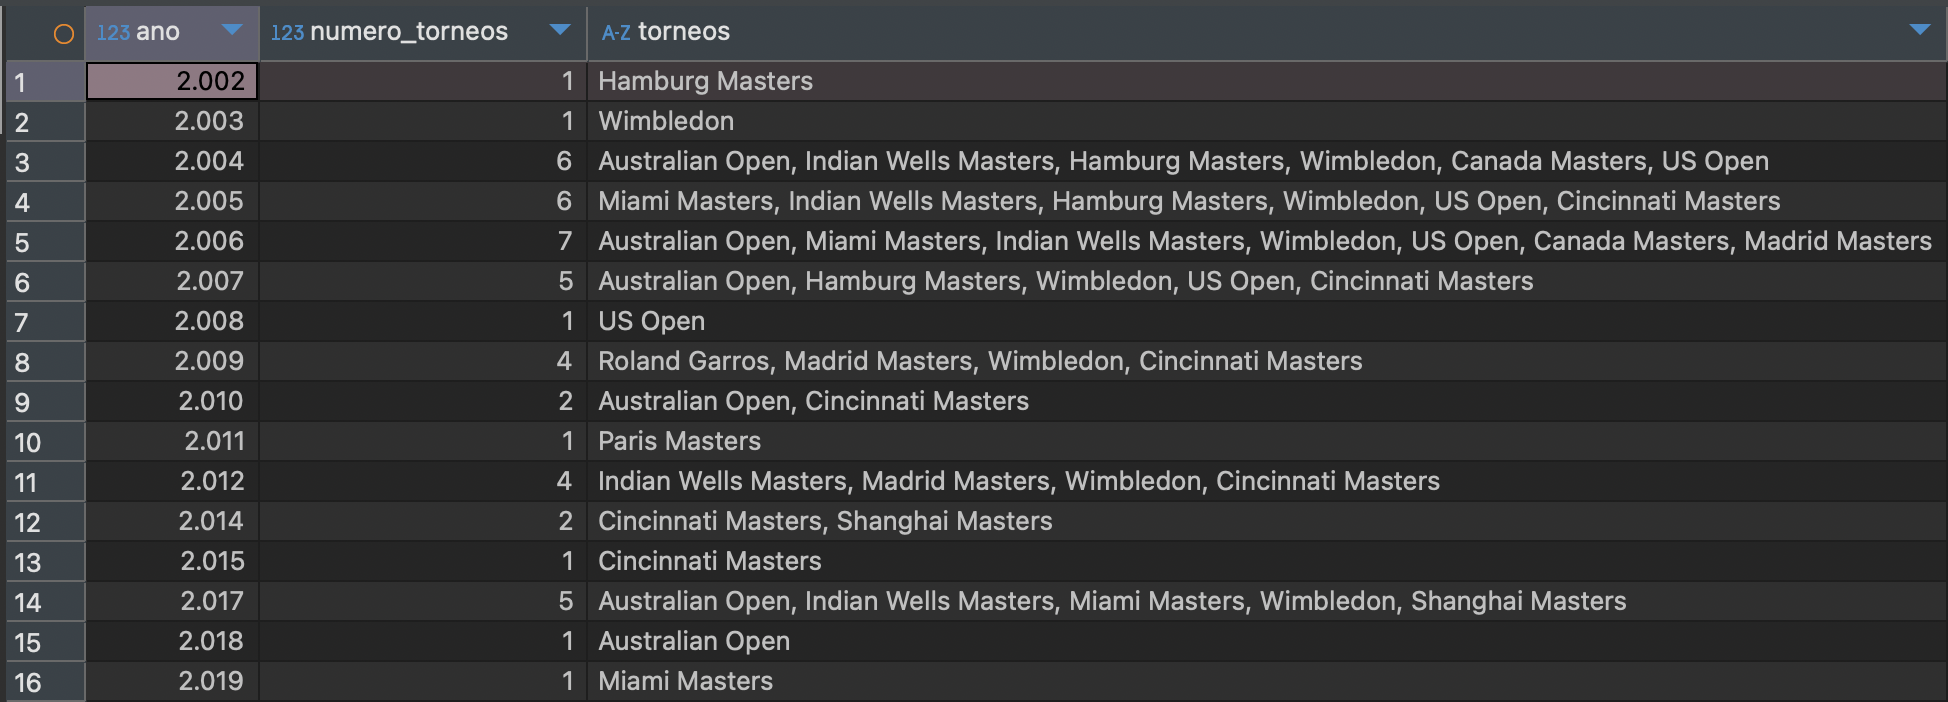
\includegraphics[width=0.8\textwidth]{fotos/q2_rel.png}
\caption{Modelo relacional Postgresql, consulta 2.}
\label{fig:q2_rel}
\end{figure}


\subsubsection{Muestra los partidos de semifinales (ronda='SF') y final (ronda = 'F') del torneo de "Roland Garros" del 2018. Para cada partido muestra la ronda, el tipo de desenlace, el nombre y apellidos del ganador y el nombre y apellidos del perdedor y el resultado con el número de juegos del ganador y del perdedor en cada set, y opcionalmente en paréntesis el número de juegos del perdedor en el tie break}

Para esta consulta necesitamos información de los partidos, los jugadores, los torneos y los sets de los partidos; como debemos distinguir entre el ganador y el perdedor, sin ningún tipo de ambigüedad, en el \texttt{from} usamos dos instancias de la tabla \texttt{jugador}, cada una con un alias distinto, por lo que estaremos haciendo el producto cartesiano de la tabla \texttt{jugador} consigo misma, así como con las tablas \texttt{partido}, \texttt{torneo} y \texttt{sets\_partido} (especificando un alias para cada una de ellas). A continuación, especificamos las condiciones de \textit{join} en el \texttt{where}, así como otras condiciones de selección:
\begin{itemize}
\item Condiciones de \textit{join} que, en global, nos permitirán seleccionar las tuplas de partidos específicos de un torneo específico en una fecha específica:
\begin{itemize}
\item El predicado \texttt{jg.id = p.ganador} sirve para unir la tabla \texttt{jugador} con la tabla \texttt{partido} mediante el atributo \texttt{id} de la tabla \texttt{jugador} y el atributo \texttt{ganador} de la tabla \texttt{partido}, haciendo una selección únicamente de las tuplas que cumplan esta condición. Esto nos permite, para cada jugador, seleccionar solo los partidos en los que ha ganado.
\item Del mismo modo, usamos el predicado \texttt{jp.id = p.perdedor} para eleccionar solo los partidos en los que ha perdido un determinado jugador. 
\item El predicado \texttt{p.fecha = sp.fecha} sirve para unir la tabla \texttt{partido} con la tabla \texttt{sets\_partido} mediante el atributo \texttt{fecha} de la tabla \texttt{partido} y el atributo \texttt{fecha} de la tabla \texttt{sets\_partido}, haciendo una selección únicamente de las tuplas que cumplan esta condición. Esto nos permite seleccionar solo los sets de los partidos que se han jugado en una fecha concreta.
\item Como la fecha anterior no es unívoca para cada partido, necesitamos una condición adicional para obtener los sets de un partido determinado. Para ello, usamos el predicado \texttt{p.num\_partido = sp.num\_partido}, que une la tabla \texttt{partido} con la tabla \texttt{sets\_partido} mediante el atributo \texttt{num\_partido} de la tabla \texttt{partido} y el atributo \texttt{num\_partido} de la tabla \texttt{sets\_partido}, haciendo una selección únicamente de las tuplas que cumplan esta condición.
\item El predicado \texttt{t.id = p.torneo} sirve para unir la tabla \texttt{torneo} con la tabla \texttt{partido} mediante el atributo \texttt{id} de la tabla \texttt{torneo} y el atributo \texttt{torneo} de la tabla \texttt{partido}, haciendo una selección únicamente de las tuplas que cumplan esta condición. Esto nos permite seleccionar solo los partidos que se han jugado en un torneo concreto.
\end{itemize}
\item Concretamente, estamos interesados en las semifinales (ronda='SF') y la final (ronda='F) del torneo de ``Roland Garros'' del 2018. Por tanto, las condiciones de selección son:
\begin{itemize}
\item El predicado \texttt{p.ronda in ('SF', 'F')} selecciona solo los partidos que han sido semifinales o finales.
\item El predicado \texttt{t.nombre = 'Roland Garros'} selecciona solo los partidos que se han jugado en el torneo ``Roland Garros''.
\item El predicado \texttt{extract(year from p.fecha) = '2018'} selecciona solo los partidos que se han jugado en el año 2018.
\end{itemize}
\end{itemize}

Ahora, para cada combinación de \texttt{p.ronda}, \texttt{p.desenlace}, \texttt{jg.nombre}, \texttt{jg.apellido}, \texttt{jp.nombre} y \texttt{jp.apellido}, tendremos una fila para cada set, donde solo variará la información de los juegos ganados y perdidos. Por tanto, agrupamos por los atributos mencionados anteriormente y, en la proyección, concatenamos los resultados de los juegos ganados y perdidos en cada set, así como el resultado final del partido, para lo que usamos la función \texttt{string\_agg()}. Como también debemos especificar la puntuación del \textit{tiebreak} (en caso de haberla), usamos un \texttt{case} para comprobar si el atributo \texttt{puntos\_tiebreak\_perdedor} es \texttt{null} o no: en caso que sea nulo, concatenamos una cadena vacia, en caso de no ser nulo, concatenamos la puntuación del \textit{tiebreak}, puesta entre paréntesis. Si bien esta es una parte de la proyección, el resto incluye simplemente la ronda, el desenlace, la fecha y los nombres y apellidos de los jugadores concatenados (un atributo para el ganador y otro para el perdedor). El código de la consulta se muestra a continuación, y el resultado se pueden ver en la figura \ref{fig:q3_rel}.

\begin{minted}[frame=single, fontsize=\small]{sql}
select p.ronda, p.desenlace, jg.nombre || ' ' || jg.apellido AS ganador, 
	jp.nombre || ' ' || jp.apellido AS perdedor, 
	STRING_AGG(sp.juegos_ganador || '-' || sp.juegos_perdedor ||
		case
		  when sp.puntos_tiebreak_perdedor is not null then 
		  	'(' || sp.puntos_tiebreak_perdedor || ')'
		  else 
		  	'' 
		end, ', ' order by sp.num_set) as resultado
from partido p, jugador jg, jugador jp, sets_partido sp, torneo t
where jg.id = p.ganador
  and jp.id = p.perdedor
  and p.fecha = sp.fecha
  and p.num_partido = sp.num_partido
  and t.id = p.torneo
  and p.ronda in ('SF', 'F')
  and t.nombre = 'Roland Garros'
  and extract(year from p.fecha) = '2018'
group by p.ronda, p.desenlace, jg.nombre, jg.apellido, jp.nombre, jp.apellido
\end{minted}

\begin{figure}[H]
\centering
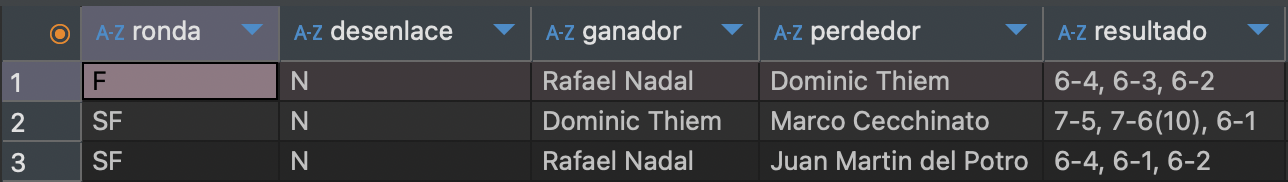
\includegraphics[width=0.7\textwidth]{fotos/q3_rel.png}
\caption{Modelo relacional Postgresql, consulta 3.}
\label{fig:q3_rel}
\end{figure}

\subsubsection{Muestra la lista de jugadores españoles (ES) que ganaron algún torneo de nivel Gran Slam (G). Para cada jugador muestra los siguientes datos resumen de todos sus partidos: número de partidos jugados, porcentaje de victorias, porcentaje de aces, porcentaje de dobles faltas, porcentaje de servicios ganados, porcentaje de restos ganados, porcentaje de break points salvados (de los sufridos en contra), porcentaje de break points ganados (de los provocados a favor)}

Esta consulta la dividiremos en dos partes: primero, buscaremos los jugadores españoles que ganaron algún torneo de nivel Grand Slam (G), y, a continuación, calcularemos los datos resumen que se piden de todos sus partidos. Para la primera parte, necesitamos información de los jugadores, los partidos y las ediciones de los torneos; comenzamos en el \texttt{from} con el producto cartesiano de las tablas \texttt{jugador}, \texttt{partido} y \texttt{edicion\_torneo} (especificando un alias para cada una de ellas). A continuación, especificamos las condiciones de \textit{join} en el \texttt{where}, así como otras condiciones de selección:
\begin{itemize}
\item Condiciones de \textit{join} que, en global, nos permitirán seleccionar las tuplas de un torneo específico:
\begin{itemize}
\item El predicado \texttt{j.id = p.ganador} sirve para unir la tabla \texttt{jugador} con la tabla \texttt{partido} mediante el atributo \texttt{id} de la tabla \texttt{jugador} y el atributo \texttt{ganador} de la tabla \texttt{partido}, haciendo una selección únicamente de las tuplas que cumplan esta condición. Esto nos permite, para cada jugador, seleccionar solo los partidos en los que ha ganado. 
\item El predicado \texttt{p.torneo = et.torneo} sirve para unir la tabla \texttt{partido} con la tabla \texttt{edicion\_torneo} mediante el atributo \texttt{torneo} de la tabla \texttt{partido} y el atributo \texttt{torneo} de la tabla \texttt{edicion\_torneo}, haciendo una selección únicamente de las tuplas que cumplan esta condición. Esto nos permite seleccionar solo los partidos que se han jugado en una edición concreta de un torneo.
\item El predicado \texttt{p.fecha = et.fecha} sirve para unir la tabla \texttt{partido} con la tabla \texttt{edicion\_torneo} mediante el atributo \texttt{fecha} de la tabla \texttt{partido} y el atributo \texttt{fecha} de la tabla \texttt{edicion\_torneo}, haciendo una selección únicamente de las tuplas que cumplan esta condición. Esto nos permite seleccionar solo los partidos que se han jugado en una fecha concreta.
\end{itemize}
\item Como de todo lo anterior solo nos interesan los partidos finales (F) de torneos de nivel Grand Slam (G) y ganados por jugadores españoles (ES), las condiciones de selección son:
\begin{itemize}
\item El predicado \texttt{p.ronda = 'F'} selecciona solo los partidos que han sido finales.
\item El predicado \texttt{et.nivel = 'G'} selecciona solo los torneos de nivel Grand Slam (G).
\item El predicado \texttt{j.pais = 'ES'} selecciona solo los jugadores españoles.
\end{itemize}
\end{itemize}

Con todo esto, obtenemos una tabla con los jugadores españoles que han ganado algún torneo de nivel Grand Slam (G), pero hay repeticion ya que estamos considerando cada edición de cada Grand Slam. Para quedarnos solo con el subconjunto que nos interesa (sin repetición), usamos un \texttt{distinct} en la proyección. Concretamente, obtenemos la proyección del \texttt{id} y el nombre completo del jugador, que concatenamos con el operador \texttt{||}, y aplicamos el \texttt{distinct} sobre la proyección. Esta tabla resultado la guardamos como \texttt{jugadores\_espanoles\_ganadores}, y la usaremos en la segunda parte de la consulta. \\

Para obtener las estadísticas resumen de cada jugador español ganador de un Grand Slam, necesitamos solo información sobre quiénes son esos jugadores y sobre los partidos que han jugado. Por tanto, en el \texttt{from} usamos la tabla \texttt{jugadores\_espanoles\_ganadores} que acabamos de crear, y la tabla \texttt{partido} (especificando un alias para cada una de ellas). A continuación, especificamos las condiciones de \textit{join} en el \texttt{where}, así como otras condiciones de selección:
\begin{itemize}
\item Condiciones de \textit{join} que, en global, nos permitirán seleccionar las tuplas de partidos de un jugador específico:
\begin{itemize}
\item El predicado \texttt{jeg.id_jugador = p.ganador or jeg.id_jugador = p.perdedor} nos permite seleccionar los partidos, tanto ganados como perdidos, en los que ha participado un jugador específico de la tabla \texttt{jugadores\_espanoles\_ganadores}.
\end{itemize}
\end{itemize}

Con esto, obtenemos una fila por cada partido de cada jugador, por lo que agrupamos por el jugador antes de agregar valores. En la proyección, obtenemos varios atributos, que redondearemos a un decimal usando \texttt{round(..., 1)}:
\begin{itemize}
\item El nombre completo del jugador, que concatenamos previamente con el operador \texttt{||}.
\item El número de partidos jugados como el conteo de los partidos en los que ha participado (\texttt{count(p.num\_partido)}).
\item El porcentaje de victorias, que calculamos como el número de partidos ganados entre el número total de partidos jugados, multiplicado por 100. Para obtener el número de partidos ganados, usamos un \texttt{case} que comprueba si el jugador es el ganador del partido o no. Esto genera una lista que contiene 1 si el jugador es el ganador y 0 si no lo es, y con \texttt{sum()} sumamos los valores de esta lista para obtener el número de partidos ganados. 
\end{itemize}

\begin{minted}[frame=single, fontsize=\small]{sql}
with jugadores_espanoles_ganadores as (
    select distinct j.id as id_jugador, j.nombre || ' ' || j.apellido as jugador
    from partido p, jugador j, edicion_torneo et 
    where p.ganador = j.id 
        and p.torneo = et.torneo 
        and p.fecha = et.fecha
        and j.pais = 'ES'
        and p.ronda = 'F'
        and et.nivel = 'G'
)

select jeg.jugador, count(p.num_partido) as partidos,
    round(100.0 * sum(case when jeg.id_jugador = p.ganador then 1 else 0 end) / count(p.num_partido), 1) as pcje_victorias, 
    round(100.0 * sum(case when jeg.id_jugador = p.ganador then p.num_aces_ganador else p.num_aces_perdedor end) / 
        nullif(sum(case when jeg.id_jugador = p.ganador then p.num_ptos_servidos_ganador  else p.num_ptos_servidos_perdedor end), 0), 1) as pcje_aces, 
    round(100.0 * sum(case when jeg.id_jugador = p.ganador then p.num_dob_faltas_ganador  else p.num_dob_faltas_perdedor  end) / 
        nullif(sum(case when jeg.id_jugador = p.ganador then p.num_ptos_servidos_ganador  else p.num_ptos_servidos_perdedor end), 0), 1) as pcje_dobles_faltas, 
    round(100.0 * sum(case when jeg.id_jugador = p.ganador then p.num_primeros_servicios_ganados_ganador + p.num_segundos_servicios_ganados_ganador 
            else p.num_primeros_servicios_ganados_perdedor + p.num_segundos_servicios_ganados_perdedor end) / 
        nullif(sum(case when jeg.id_jugador = p.ganador then p.num_ptos_servidos_ganador  else p.num_ptos_servidos_perdedor end), 0), 1) as pcje_servicios_ganados, 
    round(100.0 * sum(case when jeg.id_jugador = p.ganador 
            then p.num_ptos_servidos_perdedor - p.num_primeros_servicios_ganados_perdedor - p.num_segundos_servicios_ganados_perdedor 
            else p.num_ptos_servidos_ganador - p.num_primeros_servicios_ganados_ganador - p.num_segundos_servicios_ganados_ganador end) / 
        nullif(sum(case when jeg.id_jugador = p.ganador then p.num_ptos_servidos_perdedor else p.num_ptos_servidos_ganador end), 0), 1) as pcje_restos_ganados,
    round(100.0 * sum(case when jeg.id_jugador = p.ganador then p.num_break_salvados_ganador else p.num_break_salvados_perdedor end) / 
        nullif(sum(case when jeg.id_jugador = p.ganador then p.num_break_afrontados_ganador else p.num_break_afrontados_perdedor end), 0), 1) as pcje_breaks_salvados, 
    round(100.0 * sum(case when jeg.id_jugador = p.ganador then p.num_break_afrontados_perdedor - p.num_break_salvados_perdedor 
            else p.num_break_afrontados_ganador - p.num_break_salvados_ganador end) / 
        nullif(sum(case when jeg.id_jugador = p.ganador then p.num_break_afrontados_perdedor else p.num_break_afrontados_ganador end), 0), 1) as pcje_breaks_ganados
from jugadores_espanoles_ganadores jeg, partido p
where jeg.id_jugador = p.ganador 
	or jeg.id_jugador = p.perdedor
group by jeg.jugador
\end{minted}

\subsubsection{Lista los jugadores que fueron derrotados (en algún partido del 2018) por el rival de Rafael Nadal de la primera ronda (R128) de Roland Garros de 2018}

\begin{minted}[frame=single, fontsize=\small]{sql}
with rival_nadal as (
	select case when jg.nombre = 'Rafael' then jp.id else jg.id end as id_jugador, 
		case when jg.nombre = 'Rafael' then jp.nombre || ' ' || jp.apellido else jg.nombre || ' ' || jg.apellido end as jugador
	from partido p, jugador jg, jugador jp, edicion_torneo et, torneo t 
	where p.ganador = jg.id 
		and p.perdedor = jp.id
		and p.torneo = et.torneo 
		and p.fecha = et.fecha
		and et.torneo = t.id 
		and t.nombre = 'Roland Garros'
		and p.ronda = 'R128'
		and extract(year from p.fecha) = '2018'
		and (jg.nombre = 'Rafael' and jg.apellido = 'Nadal' or jp.nombre = 'Rafael' and jp.apellido = 'Nadal') 
)

select j.nombre || ' ' || j.apellido as jugador, j.pais as pais
from rival_nadal rn, partido p, jugador j
where rn.id_jugador = p.ganador 
	and p.perdedor = j.id
	and extract(year from p.fecha) = '2018'
\end{minted}


































\section{Datos agregados en SQL (PostgreSQL)}
(un array es homogeneo, una tupla no !!)

\subsection{Tipos compuestos}

\begin{minted}[frame=single, fontsize=\small]{sql}
create type pais_info as (
	codigo_iso2 char(2),
	codigo_iso3 char(3),
	codigo_ioc char(3),
	nombre varchar(100)
)

create type torneo_info as (
	id integer,
	nombre varchar(100),
	pais pais_info
)

create type edicion_torneo_info as (
	torneo torneo_info,
	fecha date,
	superficie varchar(20),
	tamano integer,
	nivel char(1)
)

create type set_info as (
	torneo torneo_info, --quitar
	fecha date, --quitar
	num_partido integer, --quitar
    num_set integer,
   juegos_ganador integer,
   juegos_perdedor integer,
   puntos_tiebreak_perdedor integer
)

create type jugador_stats as (
	num_aces integer,
	num_dob_faltas integer,
	num_ptos_servidos integer,
	num_primeros_servicios integer,
	num_primeros_servicios_ganados integer,
	num_segundos_servicios_ganados integer,
	num_juegos_servidos integer,
	num_break_salvados integer,
	num_break_afrontados integer
)

create type jugador_info as (
   id integer,
   nombre varchar(100),
   apellido varchar(100),
   diesto boolean,
   fecha_nacimiento date,
   pais pais_info,
   altura integer
)
\end{minted}

\begin{minted}[frame=single, fontsize=\small]{sql}
create table partidos (
  torneo edicion_torneo_info,
  fecha date,
  num_partido integer,
  num_sets integer,
  info_sets set_info array, -- array de elementos de tipo set_info
  ronda varchar(5), 
	desenlace char(1), 
	ganador jugador_info,
	perdedor jugador_info,
	ganador_stats jugador_stats,
	perdedor_stats jugador_stats
)
\end{minted}

\begin{minted}[frame=single, fontsize=\small]{sql}
insert into partidos(
torneo, fecha, num_partido, num_sets, info_sets, ronda, desenlace, ganador, perdedor, ganador_stats, perdedor_stats)
select
   -- campo 'torneo' (tipo 'torneo_info')
   case
       when t.id is null then null
       else cast((cast((t.id, t.nombre, cast((pa.codigo_iso2, pa.codigo_iso3, pa.codigo_ioc, pa.nombre) as pais_info)) as torneo_info), 
       et.fecha, et.superficie, et.tamano, et.nivel) as edicion_torneo_info)
   end as torneo,
  
   p.fecha as fecha,
   p.num_partido as num_partido,
   p.num_sets as num_sets,
  
   -- campo 'info_set' (array de 'set_info')
   array(select cast((cast((t.id, t.nombre, cast((pa.codigo_iso2, pa.codigo_iso3, pa.codigo_ioc, pa.nombre) as pais_info)) as torneo_info),
                      sp.fecha, sp.num_partido, sp.num_set, sp.juegos_ganador, sp.juegos_perdedor, sp.puntos_tiebreak_perdedor) as set_info)
         from public.sets_partido sp
         where sp.torneo = p.torneo
         	and sp.fecha = p.fecha
         	and sp.num_partido = p.num_partido
         order by sp.num_set) as info_sets,
  
   p.ronda as ronda,
   p.desenlace as desenlace,
  
   -- campo 'ganador' (tipo 'jugador_info')
   case
       when jg.id is null then null
       else cast((jg.id, jg.nombre, jg.apellido, jg.diestro, jg.fecha_nacimiento,
       		   cast((pg.codigo_iso2, pg.codigo_iso3, pg.codigo_ioc, pg.nombre) as pais_info),
       		   jg.altura) as jugador_info)
   end as ganador,
  
   -- campo 'perdedor' (tipo 'jugador_info')
   case
       when jp.id is null then null
       else cast((jp.id, jp.nombre, jp.apellido, jp.diestro, jp.fecha_nacimiento,
       		   cast((pp.codigo_iso2, pp.codigo_iso3, pp.codigo_ioc, pp.nombre) as pais_info),
       		   jp.altura) as jugador_info)
   end as perdedor,
  
   -- campo 'ganador_stats' (tipo 'jugador_stats')
   case
       when jg.id is null and jp.id is null then null
       else cast((p.num_aces_ganador, p.num_dob_faltas_ganador,
           	   p.num_ptos_servidos_ganador, p.num_primeros_servicios_ganador,
           	   p.num_primeros_servicios_ganados_ganador, p.num_segundos_servicios_ganados_ganador,
           	   p.num_juegos_servidos_ganador, p.num_break_salvados_ganador,
           	   p.num_break_afrontados_ganador) as jugador_stats)
   end as ganador_stats,
  
   -- campo 'perdedor_stats' (tipo 'jugador_stats')
   case
       when jg.id is null and jp.id is null then null
       else cast((p.num_aces_perdedor, p.num_dob_faltas_perdedor,
           	   p.num_ptos_servidos_perdedor, p.num_primeros_servicios_perdedor,
           	   p.num_primeros_servicios_ganados_perdedor, p.num_segundos_servicios_ganados_perdedor,
           	   p.num_juegos_servidos_perdedor, p.num_break_salvados_perdedor,
           	   p.num_break_afrontados_perdedor) as jugador_stats)
   end as perdedor_stats
from public.partido p join public.edicion_torneo et on et.fecha = p.fecha and et.torneo = p.torneo 
	left join public.torneo t on t.id = et.torneo
	left join public.pais pa on t.pais = pa.codigo_iso2
	left join public.jugador jg on p.ganador = jg.id
	left join public.pais pg on jg.pais = pg.codigo_iso2
	left join public.jugador jp on p.perdedor = jp.id
	left join public.pais pp on jp.pais = pp.codigo_iso2
\end{minted}





\subsubsection{Muestra todos los ganadores del torneo ``Wimbledon'' (Nombre apellidos y año). Ordena el resultado por año.}

\begin{minted}[frame=single, fontsize=\small]{sql}
select (ganador).nombre, (ganador).apellido, extract(year from fecha) as ano
from partidos
where (torneo).torneo.nombre = 'Wimbledon'
	and ronda = 'F'
order by ano
\end{minted}





\subsubsection{Muestra los años en los que Roger Federer ganó algún torneo de nivel Gran Slam (G) o Master 1000 (M). Para cada año, muestra el número de torneos y lista sus nombres (ordenados por la fecha de celebración). Ordena el resultado por el año}

\begin{minted}[frame=single, fontsize=\small]{sql}
select extract(year from (torneo).fecha) as ano, count(distinct (torneo).torneo.id) as numero_torneos, 
	string_agg((torneo).torneo.nombre, ', ' order by (torneo).fecha) as torneos
from partidos
where (torneo).nivel in ('G', 'M')
	and (ganador).nombre = 'Roger'
	and (ganador).apellido = 'Federer'
	and ronda = 'F'
group by ano
\end{minted}





\subsubsection{Muestra los partidos de semifinales (ronda='SF') y final (ronda = 'F') del torneo de "Roland Garros" del 2018. Para cada partido muestra la ronda, el tipo de desenlace, el nombre y apellidos del ganador y el nombre y apellidos del perdedor y el resultado con el número de juegos del ganador y del perdedor en cada set, y opcionalmente en paréntesis el número de juegos del perdedor en el tie break}

\begin{minted}[frame=single, fontsize=\small]{sql}
select ronda, desenlace, 
	(ganador).nombre || ' ' || (ganador).apellido as ganador,
	(perdedor).nombre || ' ' || (perdedor).apellido as perdedor, 
	(select string_agg(iset.juegos_ganador || '-' || iset.juegos_perdedor ||
	case
		when iset.puntos_tiebreak_perdedor is not null then 
			'(' || iset.puntos_tiebreak_perdedor || ')'
		else ''
	end, ', ' order by iset.num_set) 
	from unnest(info_sets) as iset) as resultado
from partidos
where ronda in ('SF', 'F')
	and (torneo).torneo.nombre = 'Roland Garros'
	and extract(year from fecha) = '2018'
\end{minted}





\subsubsection{Muestra la lista de jugadores españoles (ES) que ganaron algún torneo de nivel Gran Slam (G). Para cada jugador muestra los siguientes datos resumen de todos sus partidos: número de partidos jugados, porcentaje de victorias, porcentaje de aces, porcentaje de dobles faltas, porcentaje de servicios ganados, porcentaje de restos ganados, porcentaje de break points salvados (de los sufridos en contra), porcentaje de break points ganados (de los provocados a favor)}

\begin{minted}[frame=single, fontsize=\small]{sql}
with jugadores_espanoles_ganadores as (
    select distinct (ganador).id as id_jugador, (ganador).nombre || ' ' || (ganador).apellido AS jugador
    from partidos
    where (ganador).pais.codigo_iso2 = 'ES'
        and ronda = 'F'
        and (torneo).nivel = 'G'
)

select
    jeg.jugador,
    count(p.num_partido) as partidos,
    round(100.0 * sum(case when jeg.id_jugador = (p.ganador).id then 1 else 0 end) / count(p.num_partido), 1) as pcje_victorias,
    round(100.0 * sum(case when jeg.id_jugador = (p.ganador).id then (p.ganador_stats).num_aces else (p.perdedor_stats).num_aces end) /
        nullif(sum(case when jeg.id_jugador = (p.ganador).id then (p.ganador_stats).num_ptos_servidos else (p.perdedor_stats).num_ptos_servidos end), 0), 1) as pcje_aces,
    round(100.0 * sum(case when jeg.id_jugador = (p.ganador).id then (p.ganador_stats).num_dob_faltas else (p.perdedor_stats).num_dob_faltas end) /
        nullif(sum(case when jeg.id_jugador = (p.ganador).id then (p.ganador_stats).num_ptos_servidos else (p.perdedor_stats).num_ptos_servidos end), 0), 1) as pcje_dobles_faltas,
    round(100.0 * sum(case when jeg.id_jugador = (p.ganador).id then (p.ganador_stats).num_primeros_servicios_ganados + (p.ganador_stats).num_segundos_servicios_ganados
            else (p.perdedor_stats).num_primeros_servicios_ganados + (p.perdedor_stats).num_segundos_servicios_ganados end) /
        nullif(sum(case when jeg.id_jugador = (p.ganador).id then (p.ganador_stats).num_ptos_servidos else (p.perdedor_stats).num_ptos_servidos end), 0), 1) as pcje_servicios_ganados,
    round(100.0 * sum(case when jeg.id_jugador = (p.ganador).id
            then (p.perdedor_stats).num_ptos_servidos - (p.perdedor_stats).num_primeros_servicios_ganados - (p.perdedor_stats).num_segundos_servicios_ganados
            else (p.ganador_stats).num_ptos_servidos - (p.ganador_stats).num_primeros_servicios_ganados - (p.ganador_stats).num_segundos_servicios_ganados end) /
        nullif(sum(case when jeg.id_jugador = (p.ganador).id then (p.perdedor_stats).num_ptos_servidos else (p.ganador_stats).num_ptos_servidos end), 0), 1) as pcje_restos_ganados,
    round(100.0 * sum(case when jeg.id_jugador = (p.ganador).id then (p.ganador_stats).num_break_salvados else (p.perdedor_stats).num_break_salvados end) /
        nullif(sum(case when jeg.id_jugador = (p.ganador).id then (p.ganador_stats).num_break_afrontados else (p.perdedor_stats).num_break_afrontados end), 0), 1) as pcje_breaks_salvados,
    round(100.0 * sum(case when jeg.id_jugador = (p.ganador).id then (p.perdedor_stats).num_break_afrontados - (p.perdedor_stats).num_break_salvados
            else (p.ganador_stats).num_break_afrontados - (p.ganador_stats).num_break_salvados end) /
        nullif(sum(case when jeg.id_jugador = (p.ganador).id then (p.perdedor_stats).num_break_afrontados else (p.ganador_stats).num_break_afrontados end), 0), 1) as pcje_breaks_ganados
from jugadores_espanoles_ganadores jeg, partidos p
where jeg.id_jugador = (p.ganador).id
    or jeg.id_jugador = (p.perdedor).id
group by jeg.jugador
\end{minted}





\subsubsection{Lista los jugadores que fueron derrotados (en algún partido del 2018) por el rival de Rafael Nadal de la primera ronda (R128) de Roland Garros de 2018}

\begin{minted}[frame=single, fontsize=\small]{sql}
with rival_nadal as (
	select case when (ganador).nombre = 'Rafael' then (perdedor).nombre || ' ' || (perdedor).apellido 
						 else (ganador).nombre || ' ' || (ganador).apellido end as jugador
	from partidos 
	where (((ganador).nombre = 'Rafael' and (ganador).apellido = 'Nadal') or 
		  ((perdedor).nombre = 'Rafael' and(perdedor).apellido = 'Nadal'))
		and ronda = 'R128'
		and (torneo).torneo.nombre = 'Roland Garros'
		and extract(year from fecha) = '2018'
)

select (p.perdedor).nombre || ' ' || (p.perdedor).apellido as jugador, (p.perdedor).pais.codigo_iso2 as pais
from partidos p, rival_nadal rn
where (p.ganador).nombre || ' ' || (p.ganador).apellido = rn.jugador
	and extract(year from p.fecha) = '2018'
order by jugador
\end{minted}


































\subsection{JSON}

\begin{minted}[frame=single, fontsize=\small]{sql}
create table tenisjson as
select 
	-- columna 'jugador' como objeto json
	jsonb_build_object(
		'id', j.id, 
		'nombre', j.nombre, 
		'apellido', j.apellido, 
		'diestro', j.diestro, 
		'fecha_nacimiento', j.fecha_nacimiento, 
		'altura', j.altura
	) as jugador,
  -- columna 'pais' como objeto json
	jsonb_build_object(
		'codigo_iso2', p.codigo_iso2, 
		'codigo_iso3', p.codigo_iso3, 
		'codigo_ioc', p.codigo_ioc, 
		'nombre', p.nombre
	) as pais,
  -- columna 'partidos_ganados' como agregado json
	(select jsonb_agg(jsonb_build_object(
		'torneo', jsonb_build_object(
			'nombre', t.nombre, 
			'pais', jsonb_build_object(
				'codigo_iso2', pa.codigo_iso2, 
				'codigo_iso3', pa.codigo_iso3, 
				'codigo_ioc', pa.codigo_ioc, 
				'nombre', pa.nombre), 
			'fecha', et.fecha, 
			'superficie', et.superficie, 
			'tamano', et.tamano, 
			'nivel', et.nivel), 
		'fecha', pg.fecha, 
		'ronda', pg.ronda, 
		'desenlace', pg.desenlace, 
		'num_partido', pg.num_partido, 
		'rival', pg.perdedor, 
		'sets', (select jsonb_agg(
			jsonb_build_object(
				'num_set', sp.num_set, 
				'juegos_ganador', sp.juegos_ganador, 
				'juegos_perdedor', sp.juegos_perdedor, 
				'puntos_tiebreak_perdedor', sp.puntos_tiebreak_perdedor
			)
		) 
		from sets_partido sp 
		where sp.torneo = pg.torneo 
			and sp.fecha = pg.fecha 
			and sp.num_partido = pg.num_partido), 
		'stats', jsonb_build_object(
			'num_aces', pg.num_aces_ganador, 
			'num_dob_faltas', pg.num_dob_faltas_ganador, 
			'num_puntos_servidos', pg.num_ptos_servidos_ganador, 
			'num_primeros_servicios', pg.num_primeros_servicios_ganador, 
			'num_primeros_servicios_ganados', pg.num_primeros_servicios_ganados_ganador, 
			'num_segundos_servicios_ganados', pg.num_segundos_servicios_ganados_ganador, 
			'num_juegos_servidos', pg.num_juegos_servidos_ganador, 
			'num_break_salvados', pg.num_break_salvados_ganador, 
			'num_break_afrontados', pg.num_break_afrontados_ganador
		), 
		'stats_rival', jsonb_build_object(
			'num_aces', pg.num_aces_perdedor, 
			'num_dob_faltas', pg.num_dob_faltas_perdedor, 
			'num_puntos_servidos', pg.num_ptos_servidos_perdedor, 
			'num_primeros_servicios', pg.num_primeros_servicios_perdedor, 
			'num_primeros_servicios_ganados', pg.num_primeros_servicios_ganados_perdedor, 
			'num_segundos_servicios_ganados', pg.num_segundos_servicios_ganados_perdedor, 
			'num_juegos_servidos', pg.num_juegos_servidos_perdedor, 
			'num_break_salvados', pg.num_break_salvados_perdedor, 
			'num_break_afrontados', pg.num_break_afrontados_perdedor
		)
	)) 
	from public.partido pg 
		left join public.edicion_torneo et on pg.torneo = et.torneo and pg.fecha = et.fecha 
		left join public.torneo t on et.torneo = t.id 
		left join public.pais pa on t.pais = pa.codigo_iso2
	where pg.ganador = j.id) as partidos_ganados,
   -- columna 'partidos_perdidos' como json
	(select jsonb_agg(jsonb_build_object(
		'torneo', jsonb_build_object(
			'nombre', t.nombre, 
			'pais', jsonb_build_object(
				'codigo_iso2', pa.codigo_iso2,
				'codigo_iso3', pa.codigo_iso3,
				'codigo_ioc', pa.codigo_ioc,
				'nombre', pa.nombre
			),
			'fecha', et.fecha,
			'superficie', et.superficie,
			'tamano', et.tamano,
			'nivel', et.nivel
		),
		'fecha', pp.fecha,
		'ronda', pp.ronda,
		'desenlace', pp.desenlace,
		'num_partido', pp.num_partido,
		'rival', pp.ganador,
		'sets', (select jsonb_agg(
			jsonb_build_object(
				'num_set', sp.num_set,
				'juegos_ganador', sp.juegos_ganador,
				'juegos_perdedor', sp.juegos_perdedor,
				'puntos_tiebreak_perdedor', sp.puntos_tiebreak_perdedor
			)
		) 
		from sets_partido sp 
		where sp.torneo = pp.torneo 
			and sp.fecha = pp.fecha 
			and sp.num_partido = pp.num_partido),
		'stats', jsonb_build_object(
			'num_aces', pp.num_aces_perdedor,
			'num_dob_faltas', pp.num_dob_faltas_perdedor,
			'num_puntos_servidos', pp.num_ptos_servidos_perdedor,
			'num_primeros_servicios', pp.num_primeros_servicios_perdedor,
			'num_primeros_servicios_ganados', pp.num_primeros_servicios_ganados_perdedor,
			'num_segundos_servicios_ganados', pp.num_segundos_servicios_ganados_perdedor,
			'num_juegos_servidos', pp.num_juegos_servidos_perdedor,
			'num_break_salvados', pp.num_break_salvados_perdedor,
			'num_break_afrontados', pp.num_break_afrontados_perdedor
		),
		'stats_rival', jsonb_build_object(
			'num_aces', pp.num_aces_ganador,
			'num_dob_faltas', pp.num_dob_faltas_ganador,
			'num_puntos_servidos', pp.num_ptos_servidos_ganador,
			'num_primeros_servicios', pp.num_primeros_servicios_ganador,
			'num_primeros_servicios_ganados', pp.num_primeros_servicios_ganados_ganador,
			'num_segundos_servicios_ganados', pp.num_segundos_servicios_ganados_ganador,
			'num_juegos_servidos', pp.num_juegos_servidos_ganador,
			'num_break_salvados', pp.num_break_salvados_ganador,
			'num_break_afrontados', pp.num_break_afrontados_ganador
		)
	)) 
	from public.partido pp
		left join public.edicion_torneo et on pp.torneo = et.torneo and pp.fecha = et.fecha
		left join public.torneo t on et.torneo = t.id
		left join public.pais pa on t.pais = pa.codigo_iso2
	where pp.perdedor = j.id) as partidos_perdidos
from public.jugador j
	left join public.pais p on j.pais = p.codigo_iso2
where j.id in (select perdedor from public.partido)
	or j.id in (select ganador from public.partido)
\end{minted}





\subsubsection{Muestra todos los ganadores del torneo ``Wimbledon'' (Nombre apellidos y año). Ordena el resultado por año.}

\begin{minted}[frame=single, fontsize=\small]{sql}
select tj.jugador ->> 'nombre' as nombre, 
    tj.jugador ->> 'apellido' as apellido, 
    extract(year from (pg ->> 'fecha')::date) as ano
from tenisjson tj, jsonb_array_elements(partidos_ganados) as partidos(pg)
where pg ->> 'ronda' = 'F' 
    and pg -> 'torneo' ->> 'nombre' = 'Wimbledon'
order by ano
\end{minted}





\subsubsection{Muestra los años en los que Roger Federer ganó algún torneo de nivel Gran Slam (G) o Master 1000 (M). Para cada año, muestra el número de torneos y lista sus nombres (ordenados por la fecha de celebración). Ordena el resultado por el año}

\begin{minted}[frame=single, fontsize=\small]{sql}
select extract(year from (pg -> 'torneo' ->> 'fecha')::date) as ano,
    count(distinct pg -> 'torneo'->>'nombre') as numero_torneos,
    string_agg(pg -> 'torneo'->>'nombre', ', ' order by pg -> 'torneo' ->> 'fecha') as torneos
from tenisjson tj, jsonb_array_elements(partidos_ganados) as partidos(pg)
where tj.jugador ->> 'nombre' = 'Roger'
    and tj.jugador ->> 'apellido' = 'Federer'
    and pg ->> 'ronda' = 'F'
    and pg -> 'torneo'->>'nivel' in ('G', 'M')
group by ano
order by ano
\end{minted}





\subsubsection{Muestra los partidos de semifinales (ronda='SF') y final (ronda = 'F') del torneo de "Roland Garros" del 2018. Para cada partido muestra la ronda, el tipo de desenlace, el nombre y apellidos del ganador y el nombre y apellidos del perdedor y el resultado con el número de juegos del ganador y del perdedor en cada set, y opcionalmente en paréntesis el número de juegos del perdedor en el tie break}

\begin{minted}[frame=single, fontsize=\small]{sql}
select pg ->> 'ronda' as ronda, pg ->> 'desenlace' as desenlace, 
	(tj.jugador ->> 'nombre')::text || ' ' || (tj.jugador ->> 'apellido')::text as ganador, 
	(tjr.jugador ->> 'nombre')::text || ' ' || (tjr.jugador ->> 'apellido')::text as perdedor, 
	string_agg((s ->> 'juegos_ganador')::text || '-' || (s ->> 'juegos_perdedor')::text || 
		case when s ->> 'puntos_tiebreak_perdedor' is not null 
			then '(' || (s ->> 'puntos_tiebreak_perdedor')::text || ')' 
			else '' end, ', ' order by s ->> 'num_set') as resultado
from tenisjson tj, jsonb_array_elements(tj.partidos_ganados) as partidos(pg), 
	jsonb_array_elements(pg -> 'sets') as setss(s), tenisjson tjr
where pg ->'torneo' ->> 'nombre' = 'Roland Garros'
    and extract(year from (pg ->> 'fecha')::date) = 2018
    and pg ->> 'ronda' in ('SF', 'F')
    and tjr.jugador->>'id' = pg ->> 'rival'
group by pg ->> 'ronda', pg ->> 'desenlace', 
	tj.jugador ->> 'nombre', tj.jugador ->> 'apellido', 
	tjr.jugador ->> 'nombre', tjr.jugador ->> 'apellido', pg ->> 'fecha'
\end{minted}





\subsubsection{Muestra la lista de jugadores españoles (ES) que ganaron algún torneo de nivel Gran Slam (G). Para cada jugador muestra los siguientes datos resumen de todos sus partidos: número de partidos jugados, porcentaje de victorias, porcentaje de aces, porcentaje de dobles faltas, porcentaje de servicios ganados, porcentaje de restos ganados, porcentaje de break points salvados (de los sufridos en contra), porcentaje de break points ganados (de los provocados a favor)}

\begin{minted}[frame=single, fontsize=\small]{sql}
with jugadores_espanoles_ganadores as (
    select distinct (tj.jugador ->> 'id')::integer as id_jugador, 
    	(tj.jugador ->> 'nombre')::text || ' ' || (tj.jugador ->> 'apellido')::text as jugador
    from tenisjson tj, jsonb_array_elements(partidos_ganados) as partidos(pg)
    where tj.pais ->> 'codigo_iso2' = 'ES'
        and pg ->> 'ronda' = 'F'
        and pg -> 'torneo' ->> 'nivel' = 'G'
)

select jeg.jugador,
    count(*) as partidos,
    round(100.0 * count(case when pg ->> 'rival' = jeg.id_jugador::text then null else 1 end)::numeric / count(*), 1) as pcje_victorias,
    round(100.0 * sum(case when pg ->> 'rival' = jeg.id_jugador::text 
    	then (pg -> 'stats_rival' ->> 'num_aces')::numeric 
    	else (pg -> 'stats' ->> 'num_aces')::numeric end) / 
    	nullif(sum(case when pg ->> 'rival' = jeg.id_jugador::text 
    		then (pg -> 'stats_rival' ->> 'num_puntos_servidos')::numeric 
    		else (pg->'stats'->>'num_puntos_servidos')::numeric end), 0), 1) as pcje_aces,
    round(100.0 * sum(case when pg ->> 'rival' = jeg.id_jugador::text 
    	then (pg -> 'stats_rival' ->> 'num_dob_faltas')::numeric 
    	else (pg -> 'stats' ->> 'num_dob_faltas')::numeric end) / 
    	nullif(sum(case when pg ->> 'rival' = jeg.id_jugador::text 
    		then (pg -> 'stats_rival' ->> 'num_puntos_servidos')::numeric 
    		else (pg -> 'stats' ->> 'num_puntos_servidos')::numeric end), 0), 1) as pcje_dobles_faltas,
    round(100.0 * sum(case when pg ->> 'rival' = jeg.id_jugador::text 
    	then (pg -> 'stats_rival' ->> 'num_primeros_servicios_ganados')::numeric + (pg -> 'stats_rival' ->> 'num_segundos_servicios_ganados')::numeric 
    	else (pg -> 'stats' ->> 'num_primeros_servicios_ganados')::numeric + (pg -> 'stats' ->> 'num_segundos_servicios_ganados')::numeric end) / 
    	nullif(sum(case when pg ->> 'rival' = jeg.id_jugador::text 
    		then (pg -> 'stats_rival' ->> 'num_puntos_servidos')::numeric 
    		else (pg -> 'stats' ->> 'num_puntos_servidos')::numeric end), 0), 1) as pcje_servicios_ganados,
    round(100.0 * sum(case when pg ->> 'rival' = jeg.id_jugador::text 
    	then (pg -> 'stats' ->> 'num_puntos_servidos')::numeric - (pg -> 'stats' ->> 'num_primeros_servicios_ganados')::numeric - 
    		 (pg -> 'stats' ->> 'num_segundos_servicios_ganados')::numeric 
    	else (pg -> 'stats_rival' ->> 'num_puntos_servidos')::numeric - (pg -> 'stats_rival' ->> 'num_primeros_servicios_ganados')::numeric - 
    		 (pg -> 'stats_rival' ->> 'num_segundos_servicios_ganados')::numeric end) / 	
    	nullif(sum(case when pg ->> 'rival' = jeg.id_jugador::text 
    		then (pg -> 'stats' ->> 'num_puntos_servidos')::numeric 
    		else (pg -> 'stats_rival' ->> 'num_puntos_servidos')::numeric end), 0), 1) as pcje_restos_ganados,
    round(100.0 * sum(case when pg ->> 'rival' = jeg.id_jugador::text 
    	then (pg->'stats_rival'->>'num_break_salvados')::numeric 
    	else (pg -> 'stats' ->> 'num_break_salvados')::numeric end) / 
    	nullif(sum(case when pg ->> 'rival' = jeg.id_jugador::text 
    		then (pg -> 'stats_rival' ->> 'num_break_afrontados')::numeric 
    		else (pg -> 'stats' ->> 'num_break_afrontados')::numeric end), 0), 1) as pcje_breaks_salvados,
    round(100.0 * sum(case when pg ->> 'rival' = jeg.id_jugador::text 
    	then (pg -> 'stats' ->> 'num_break_afrontados')::numeric - (pg -> 'stats' ->> 'num_break_salvados')::numeric
    	else (pg -> 'stats_rival' ->> 'num_break_afrontados')::numeric - (pg -> 'stats_rival' ->> 'num_break_salvados')::numeric end) / 
    	nullif(sum(case when pg ->> 'rival' = jeg.id_jugador::text 
    		then (pg -> 'stats' ->> 'num_break_afrontados')::numeric 
    		else (pg -> 'stats_rival' ->> 'num_break_afrontados')::numeric end), 0), 1) as pcje_breaks_ganados
from jugadores_espanoles_ganadores jeg, tenisjson tj, 
	jsonb_array_elements(tj.partidos_ganados) as partidos(pg)
where (tj.jugador ->> 'id')::integer = jeg.id_jugador 
	or pg ->> 'rival' = jeg.id_jugador::text
group by jeg.jugador
\end{minted}





\subsubsection{Lista los jugadores que fueron derrotados (en algún partido del 2018) por el rival de Rafael Nadal de la primera ronda (R128) de Roland Garros de 2018}

\begin{minted}[frame=single, fontsize=\small]{sql}
with rival_nadal as (
	select case when tj.jugador ->> 'nombre' = 'Rafael' 
			then (pg ->> 'rival')::integer  
			else (tj.jugador ->> 'id')::integer end as id_jugador,
		case when tj.jugador ->> 'nombre' = 'Rafael' 
			then (tjr.jugador ->> 'nombre')::text || ' ' || (tjr.jugador ->> 'apellido')::text 
			else (tj.jugador ->> 'nombre')::text || ' ' || (tj.jugador ->> 'apellido')::text end as jugador
	from tenisjson tj, jsonb_array_elements(tj.partidos_ganados) as partidos(pg), tenisjson tjr
    where pg -> 'torneo' ->> 'nombre' = 'Roland Garros' 
    	and pg ->> 'ronda' = 'R128'
		and extract(year from (pg ->> 'fecha')::date) = 2018
        and tjr.jugador->>'id' = pg ->> 'rival'
        and ((tj.jugador ->> 'nombre' = 'Rafael' and tj.jugador ->> 'apellido' = 'Nadal') 
        	or (tjr.jugador ->> 'nombre' = 'Rafael' and tjr.jugador ->> 'apellido' = 'Nadal'))
)

select tj.jugador->>'nombre' || ' ' || (tj.jugador->>'apellido')::text as jugador, 
	tj.pais->>'codigo_iso2' as pais
from rival_nadal rn, tenisjson tj, jsonb_array_elements(tj.partidos_perdidos) as partidos(pg)
where rn.id_jugador = (pg->>'rival')::integer 
	and extract(year from (pg->>'fecha')::date) = 2018
\end{minted}


































\section{Bases de datos distribuidas con SQL (CITUS Data)}

\subsubsection{Muestra todos los ganadores del torneo ``Wimbledon'' (Nombre apellidos y año). Ordena el resultado por año.}

\begin{lstlisting}[language=SQL]
-- Q1
\end{lstlisting}





\subsubsection{Muestra los años en los que Roger Federer ganó algún torneo de nivel Gran Slam (G) o Master 1000 (M). Para cada año, muestra el número de torneos y lista sus nombres (ordenados por la fecha de celebración). Ordena el resultado por el año}

\begin{lstlisting}[language=SQL]
-- Q2
\end{lstlisting}





\subsubsection{Muestra los partidos de semifinales (ronda='SF') y final (ronda = 'F') del torneo de "Roland Garros" del 2018. Para cada partido muestra la ronda, el tipo de desenlace, el nombre y apellidos del ganador y el nombre y apellidos del perdedor y el resultado con el número de juegos del ganador y del perdedor en cada set, y opcionalmente en paréntesis el número de juegos del perdedor en el tie break}

\begin{lstlisting}[language=SQL]
-- Q3
\end{lstlisting}





\subsubsection{Muestra la lista de jugadores españoles (ES) que ganaron algún torneo de nivel Gran Slam (G). Para cada jugador muestra los siguientes datos resumen de todos sus partidos: número de partidos jugados, porcentaje de victorias, porcentaje de aces, porcentaje de dobles faltas, porcentaje de servicios ganados, porcentaje de restos ganados, porcentaje de break points salvados (de los sufridos en contra), porcentaje de break points ganados (de los provocados a favor)}

\begin{lstlisting}[language=SQL]
-- Q4
\end{lstlisting}





\subsubsection{Lista los jugadores que fueron derrotados (en algún partido del 2018) por el rival de Rafael Nadal de la primera ronda (R128) de Roland Garros de 2018}

\begin{lstlisting}[language=SQL]
-- Q5
\end{lstlisting}


































\section{Bases de datos NoSQL: Documentales (MongoDB)}

\subsubsection{Muestra todos los ganadores del torneo ``Wimbledon'' (Nombre apellidos y año). Ordena el resultado por año.}

\begin{lstlisting}[language=SQL]
-- Q1
\end{lstlisting}





\subsubsection{Muestra los años en los que Roger Federer ganó algún torneo de nivel Gran Slam (G) o Master 1000 (M). Para cada año, muestra el número de torneos y lista sus nombres (ordenados por la fecha de celebración). Ordena el resultado por el año}

\begin{lstlisting}[language=SQL]
-- Q2
\end{lstlisting}





\subsubsection{Muestra los partidos de semifinales (ronda='SF') y final (ronda = 'F') del torneo de "Roland Garros" del 2018. Para cada partido muestra la ronda, el tipo de desenlace, el nombre y apellidos del ganador y el nombre y apellidos del perdedor y el resultado con el número de juegos del ganador y del perdedor en cada set, y opcionalmente en paréntesis el número de juegos del perdedor en el tie break}

\begin{lstlisting}[language=SQL]
-- Q3
\end{lstlisting}





\subsubsection{Muestra la lista de jugadores españoles (ES) que ganaron algún torneo de nivel Gran Slam (G). Para cada jugador muestra los siguientes datos resumen de todos sus partidos: número de partidos jugados, porcentaje de victorias, porcentaje de aces, porcentaje de dobles faltas, porcentaje de servicios ganados, porcentaje de restos ganados, porcentaje de break points salvados (de los sufridos en contra), porcentaje de break points ganados (de los provocados a favor)}

\begin{lstlisting}[language=SQL]
-- Q4
\end{lstlisting}





\subsubsection{Lista los jugadores que fueron derrotados (en algún partido del 2018) por el rival de Rafael Nadal de la primera ronda (R128) de Roland Garros de 2018}

\begin{lstlisting}[language=SQL]
-- Q5
\end{lstlisting}


































\section{Bases de datos NoSQL: Grafos (Neo4j)}

\subsection{Creación de índices}

\begin{lstlisting}[language=Cypher]
CREATE INDEX IF NOT EXISTS FOR (j:Jugador) ON (j.id);
CREATE INDEX IF NOT EXISTS FOR (et:EdicionTorneo) ON (et.torneo, et.fecha);
CREATE INDEX IF NOT EXISTS FOR (p:Partido) ON (p.num_partido, p.fecha);
CREATE INDEX IF NOT EXISTS FOR (p:Pais) ON (p.codigo_iso2);
CREATE INDEX IF NOT EXISTS FOR (t:Torneo) ON (t.id);
CREATE INDEX partido_fecha_num IF NOT EXISTS FOR (p:Partido) ON (p.num_partido, p.fecha);
\end{lstlisting}

\subsection{Carga de datos con JBDC}

\begin{lstlisting}[language=Cypher]
// cargamos los paises
WITH "jdbc:postgresql://localhost:5432/tenis?user=alumnogreibd&password=greibd2021" as url
CALL apoc.load.jdbc(url, "SELECT codigo_iso2, codigo_iso3, codigo_ioc, nombre FROM pais") YIELD row
CREATE (p:Pais {
codigo_iso2: row.codigo_iso2,
codigo_iso3: row.codigo_iso3,
codigo_ioc: row.codigo_ioc,
nombre: row.nombre
});

// cargamos los jugadores
WITH "jdbc:postgresql://localhost:5432/tenis?user=alumnogreibd&password=greibd2021" AS url
CALL apoc.load.jdbc(url, 
"SELECT id, nombre, apellido, diestro, fecha_nacimiento, pais, altura FROM jugador") YIELD row
MATCH (pa:Pais {codigo_iso2: row.pais})
CREATE (j:Jugador {
    id: row.id,
    nombre: row.nombre,
    apellido: row.apellido,
    diestro: row.diestro,
    fecha_nacimiento: row.fecha_nacimiento,
    altura: row.altura
})
CREATE (j)-[:REPRESENTA_A]->(pa);

// cargamos los torneos
WITH "jdbc:postgresql://localhost:5432/tenis?user=alumnogreibd&password=greibd2021" AS url
CALL apoc.load.jdbc(url,
"SELECT id, nombre, pais FROM torneo") YIELD row
CREATE (t:Torneo {
    id: row.id,
    nombre: row.nombre
})
WITH t, row
OPTIONAL MATCH (pa:Pais {codigo_iso2: row.pais})
WITH t, pa
WHERE pa IS NOT NULL
CREATE (t)-[:SE_CELEBRA_EN]->(pa);

// cargamos las ediciones de los torneos
WITH "jdbc:postgresql://localhost:5432/tenis?user=alumnogreibd&password=greibd2021" AS url
CALL apoc.load.jdbc(url,
"SELECT torneo, fecha, superficie, tamano, nivel FROM edicion_torneo") YIELD row
MATCH (t:Torneo {id: row.torneo})
CREATE (et:EdicionTorneo {
    fecha: row.fecha,
    superficie: row.superficie,
    tamano: row.tamano,
    nivel: row.nivel,
    torneo: row.torneo
})
CREATE (et)-[:EDICION_DE]->(t);

// cargamos los partidos
WITH "jdbc:postgresql://localhost:5432/tenis?user=alumnogreibd&password=greibd2021" AS url
CALL apoc.load.jdbc(url,
"SELECT p.torneo, p.fecha, p.num_partido, p.num_sets, p.ronda, p.desenlace,
p.ganador, p.perdedor,
p.num_aces_ganador, p.num_dob_faltas_ganador, p.num_ptos_servidos_ganador,
p.num_primeros_servicios_ganador, p.num_primeros_servicios_ganados_ganador,
p.num_segundos_servicios_ganados_ganador, p.num_juegos_servidos_ganador,
p.num_break_salvados_ganador, p.num_break_afrontados_ganador,
p.num_aces_perdedor, p.num_dob_faltas_perdedor, p.num_ptos_servidos_perdedor,
p.num_primeros_servicios_perdedor, p.num_primeros_servicios_ganados_perdedor,
p.num_segundos_servicios_ganados_perdedor, p.num_juegos_servidos_perdedor,
p.num_break_salvados_perdedor, p.num_break_afrontados_perdedor
FROM partido p
WHERE p.fecha IS NOT NULL AND p.torneo IS NOT NULL
ORDER BY p.fecha, p.torneo, p.num_partido
LIMIT 10000 OFFSET 0") YIELD row

// creamos el partido independientemente de las referencias
CREATE (p:Partido {
num_partido: row.num_partido,
fecha: row.fecha,
num_sets: row.num_sets,
ronda: row.ronda,
desenlace: row.desenlace,
torneo_id: row.torneo // Guardamos la referencia al torneo aunque no exista el nodo
})

// vinculamos con el torneo si existe
WITH p, row
OPTIONAL MATCH (t:Torneo {id: row.torneo})
WITH p, row, t
WHERE t IS NOT NULL
CREATE (p)-[:SE_JUEGA_EN]->(t)

// vinculamos con el ganador si existe
WITH p, row
OPTIONAL MATCH (ganador:Jugador {id: toInteger(row.ganador)})
WITH p, row, ganador
WHERE ganador IS NOT NULL
CREATE (p)-[:GANADO_POR {
num_aces: row.num_aces_ganador,
num_dob_faltas: row.num_dob_faltas_ganador,
num_ptos_servidos: row.num_ptos_servidos_ganador,
num_primeros_servicios: row.num_primeros_servicios_ganador,
num_primeros_servicios_ganados: row.num_primeros_servicios_ganados_ganador,
num_segundos_servicios_ganados: row.num_segundos_servicios_ganados_ganador,
num_juegos_servidos: row.num_juegos_servidos_ganador,
num_break_salvados: row.num_break_salvados_ganador,
num_break_afrontados: row.num_break_afrontados_ganador
}]->(ganador)

// vinculamos con el perdedor si existe
WITH p, row
OPTIONAL MATCH (perdedor:Jugador {id: toInteger(row.perdedor)})
WITH p, row, perdedor
WHERE perdedor IS NOT NULL
CREATE (p)-[:PERDIDO_POR {
num_aces: row.num_aces_perdedor,
num_dob_faltas: row.num_dob_faltas_perdedor,
num_ptos_servidos: row.num_ptos_servidos_perdedor,
num_primeros_servicios: row.num_primeros_servicios_perdedor,
num_primeros_servicios_ganados: row.num_primeros_servicios_ganados_perdedor,
num_segundos_servicios_ganados: row.num_segundos_servicios_ganados_perdedor,
num_juegos_servidos: row.num_juegos_servidos_perdedor,
num_break_salvados: row.num_break_salvados_perdedor,
num_break_afrontados: row.num_break_afrontados_perdedor
}]->(perdedor);

// cargamos los sets de los partidos
WITH "jdbc:postgresql://localhost:5432/tenis?user=alumnogreibd&password=greibd2021" AS url
CALL apoc.load.jdbc(url,
"SELECT * FROM sets_partido LIMIT 10000 OFFSET 0") YIELD row
OPTIONAL MATCH (p:Partido {num_partido: row.num_partido, fecha: row.fecha})
WITH row, p
WHERE p IS NOT NULL
CREATE (sp:SetPartido {
num_set: row.num_set,
juegos_ganador: row.juegos_ganador,
juegos_perdedor: row.juegos_perdedor,
puntos_tiebreak_perdedor: row.puntos_tiebreak_perdedor
})
CREATE (sp)-[:PERTENECE_A]->(p);
\end{lstlisting}

\subsubsection{Muestra todos los ganadores del torneo ``Wimbledon'' (Nombre apellidos y año). Ordena el resultado por año.}

\begin{lstlisting}[language=Cypher]
MATCH (j:Jugador)-[gp:GANADO_POR]-(p:Partido)-[:SE_JUEGA_EN]->(t:Torneo)
WHERE t.nombre = 'Wimbledon'
AND p.ronda = 'F'
RETURN j.nombre AS nombre,
j.apellido AS apellido,
substring(toString(p.fecha), 0, 4) AS ano
ORDER BY ano;
\end{lstlisting}





\subsubsection{Muestra los años en los que Roger Federer ganó algún torneo de nivel Gran Slam (G) o Master 1000 (M). Para cada año, muestra el número de torneos y lista sus nombres (ordenados por la fecha de celebración). Ordena el resultado por el año}

\begin{lstlisting}[language=Cypher]
MATCH (j:Jugador)-[:GANADO_POR]-(p:Partido)-[:SE_JUEGA_EN]->(t:Torneo)
MATCH (et:EdicionTorneo)-[:EDICION_DE]->(t)
WHERE j.nombre = 'Roger'
AND j.apellido = 'Federer'
AND p.ronda = 'F'
AND et.nivel IN ['G', 'M']
AND et.fecha = p.fecha
AND et.torneo = t.id
WITH substring(toString(p.fecha), 0, 4) AS ano,
collect(DISTINCT t.nombre) AS torneos_nombres,
count(DISTINCT t) AS num_torneos
RETURN ano,
num_torneos,
reduce(s = head(torneos_nombres), x IN tail(torneos_nombres) | s + ', ' + x) AS torneos
ORDER BY ano;
\end{lstlisting}





\subsubsection{Muestra los partidos de semifinales (ronda='SF') y final (ronda = 'F') del torneo de "Roland Garros" del 2018. Para cada partido muestra la ronda, el tipo de desenlace, el nombre y apellidos del ganador y el nombre y apellidos del perdedor y el resultado con el número de juegos del ganador y del perdedor en cada set, y opcionalmente en paréntesis el número de juegos del perdedor en el tie break}

\begin{lstlisting}[language=Cypher]
MATCH (jg:Jugador)-[:GANADO_POR]-(p:Partido)-[:PERDIDO_POR]-(jp:Jugador),
(p)-[:SE_JUEGA_EN]->(t:Torneo),
(sp:SetPartido)-[:PERTENECE_A]->(p)
WHERE t.nombre = 'Roland Garros'
AND p.ronda IN ['SF', 'F']
AND substring(toString(p.fecha), 0, 4) = '2018'
WITH p, jg, jp, sp
ORDER BY sp.num_set
WITH p, jg, jp,
collect(sp.juegos_ganador + '-' + sp.juegos_perdedor +
CASE sp.puntos_tiebreak_perdedor
WHEN null THEN ''
ELSE '(' + toString(sp.puntos_tiebreak_perdedor) + ')'
END) as sets
RETURN p.ronda as ronda,
p.desenlace as desenlace,
jg.nombre + ' ' + jg.apellido as ganador,
jp.nombre + ' ' + jp.apellido as perdedor,
reduce(s = head(sets), x IN tail(sets) | s + ', ' + x) as resultado
ORDER BY p.fecha;
\end{lstlisting}





\subsubsection{Muestra la lista de jugadores españoles (ES) que ganaron algún torneo de nivel Gran Slam (G). Para cada jugador muestra los siguientes datos resumen de todos sus partidos: número de partidos jugados, porcentaje de victorias, porcentaje de aces, porcentaje de dobles faltas, porcentaje de servicios ganados, porcentaje de restos ganados, porcentaje de break points salvados (de los sufridos en contra), porcentaje de break points ganados (de los provocados a favor)}

\begin{lstlisting}[language=Cypher]
// Primero identificamos los jugadores espanoles que han ganado finales de Grand Slam
MATCH (j:Jugador)-[:REPRESENTA_A]->(p:Pais {codigo_iso2: 'ES'})
MATCH (j)-[:GANADO_POR]-(partido:Partido)-[:SE_JUEGA_EN]->(t:Torneo)
MATCH (et:EdicionTorneo)-[:EDICION_DE]->(t)
WHERE partido.ronda = 'F'
AND et.nivel = 'G'
AND et.fecha = partido.fecha
AND et.torneo = t.id
WITH DISTINCT j.id as id_jugador, j.nombre + ' ' + j.apellido as jugador


// Ahora calculamos todas las estadisticas para estos jugadores
MATCH (j:Jugador)
WHERE j.id = id_jugador
MATCH (p:Partido)
MATCH (j)-[r:GANADO_POR|PERDIDO_POR]-(p)
WITH jugador, p, j, r, type(r) as tipo,
CASE type(r) WHEN 'GANADO_POR' THEN 1 ELSE 0 END as es_ganador,
CASE type(r)
WHEN 'GANADO_POR' THEN r.num_aces
ELSE r.num_aces END as aces,
CASE type(r)
WHEN 'GANADO_POR' THEN r.num_ptos_servidos
ELSE r.num_ptos_servidos END as ptos_servidos,
CASE type(r)
WHEN 'GANADO_POR' THEN r.num_dob_faltas
ELSE r.num_dob_faltas END as dobles_faltas,
CASE type(r)
WHEN 'GANADO_POR' THEN r.num_primeros_servicios_ganados + r.num_segundos_servicios_ganados
ELSE r.num_primeros_servicios_ganados + r.num_segundos_servicios_ganados END as servicios_ganados,
// Para restos ganados necesitamos el rival
CASE type(r)
WHEN 'GANADO_POR' THEN [(p)-[rp:PERDIDO_POR]-() | rp.num_ptos_servidos - rp.num_primeros_servicios_ganados - rp.num_segundos_servicios_ganados][0]
ELSE [(p)-[rg:GANADO_POR]-() | rg.num_ptos_servidos - rg.num_primeros_servicios_ganados - rg.num_segundos_servicios_ganados][0] END as restos_ganados,
CASE type(r)
WHEN 'GANADO_POR' THEN [(p)-[rp:PERDIDO_POR]-() | rp.num_ptos_servidos][0]
ELSE [(p)-[rg:GANADO_POR]-() | rg.num_ptos_servidos][0] END as ptos_servidos_rival,
CASE type(r)
WHEN 'GANADO_POR' THEN r.num_break_salvados
ELSE r.num_break_salvados END as breaks_salvados,
CASE type(r)
WHEN 'GANADO_POR' THEN r.num_break_afrontados
ELSE r.num_break_afrontados END as breaks_afrontados,
CASE type(r)
WHEN 'GANADO_POR' THEN [(p)-[rp:PERDIDO_POR]-() | rp.num_break_afrontados - rp.num_break_salvados][0]
ELSE [(p)-[rg:GANADO_POR]-() | rg.num_break_afrontados - rg.num_break_salvados][0] END as breaks_ganados,
CASE type(r)
WHEN 'GANADO_POR' THEN [(p)-[rp:PERDIDO_POR]-() | rp.num_break_afrontados][0]
ELSE [(p)-[rg:GANADO_POR]-() | rg.num_break_afrontados][0] END as breaks_rival
WITH jugador,
count(p) as partidos,
100.0 * sum(es_ganador) / count(p) as pcje_victorias,
CASE WHEN sum(ptos_servidos) = 0 THEN 0
ELSE 100.0 * sum(aces) / sum(ptos_servidos) END as pcje_aces,
CASE WHEN sum(ptos_servidos) = 0 THEN 0
ELSE 100.0 * sum(dobles_faltas) / sum(ptos_servidos) END as pcje_dobles_faltas,
CASE WHEN sum(ptos_servidos) = 0 THEN 0
ELSE 100.0 * sum(servicios_ganados) / sum(ptos_servidos) END as pcje_servicios_ganados,
CASE WHEN sum(ptos_servidos_rival) = 0 THEN 0
ELSE 100.0 * sum(restos_ganados) / sum(ptos_servidos_rival) END as pcje_restos_ganados,
CASE WHEN sum(breaks_afrontados) = 0 THEN 0
ELSE 100.0 * sum(breaks_salvados) / sum(breaks_afrontados) END as pcje_breaks_salvados,
CASE WHEN sum(breaks_rival) = 0 THEN 0
ELSE 100.0 * sum(breaks_ganados) / sum(breaks_rival) END as pcje_breaks_ganados
RETURN
jugador,
partidos,
round(pcje_victorias, 1) as pcje_victorias,
round(pcje_aces, 1) as pcje_aces,
round(pcje_dobles_faltas, 1) as pcje_dobles_faltas,
round(pcje_servicios_ganados, 1) as pcje_servicios_ganados,
round(pcje_restos_ganados, 1) as pcje_restos_ganados,
round(pcje_breaks_salvados, 1) as pcje_breaks_salvados,
round(pcje_breaks_ganados, 1) as pcje_breaks_ganados
ORDER BY jugador;
\end{lstlisting}





\subsubsection{Lista los jugadores que fueron derrotados (en algún partido del 2018) por el rival de Rafael Nadal de la primera ronda (R128) de Roland Garros de 2018}

\begin{lstlisting}[language=Cypher]
// Primero encontramos al rival de Nadal en Roland Garros 2018 R128
MATCH (nadal:Jugador {nombre: 'Rafael', apellido: 'Nadal'})
MATCH (rival:Jugador)
MATCH (p:Partido)-[:SE_JUEGA_EN]->(t:Torneo {nombre: 'Roland Garros'})
WHERE p.ronda = 'R128'
AND substring(toString(p.fecha), 0, 4) = '2018'
AND ((nadal)-[:GANADO_POR]-(p)-[:PERDIDO_POR]-(rival) OR
(nadal)-[:PERDIDO_POR]-(p)-[:GANADO_POR]-(rival))


// Ahora buscamos los partidos donde este rival perdio en 2018
WITH rival
MATCH (rival)-[:GANADO_POR]-(derrotas:Partido)-[:PERDIDO_POR]-(perdedor:Jugador)
WHERE substring(toString(derrotas.fecha), 0, 4) = '2018'
MATCH (perdedor)-[:REPRESENTA_A]->(pais:Pais)
RETURN DISTINCT
perdedor.nombre + ' ' + perdedor.apellido as jugador,
pais.codigo_iso2 as pais
ORDER BY jugador;
\end{lstlisting}
    
    


\end{document}
